%%%%%%%%%%%%%%%%%%%%%%%%%%%%%%%%%%%%%%%%%%%%%%%%%%%%%%%%%%%%
%%  This Beamer template was created by Cameron Bracken.
%%  Anyone can freely use or modify it for any purpose
%%  without attribution.
%%
%%  Last Modified: January 9, 2009
%%

\documentclass[xcolor=x11names,compress]{beamer}

%% General document %%%%%%%%%%%%%%%%%%%%%%%%%%%%%%%%%%
\usepackage[utf8]{inputenc}
\usepackage[ngerman]{babel}
\usepackage{graphicx}
\usepackage{color}
\usepackage{tikz}
\usepackage{tabularx}
\usepackage[skins]{tcolorbox}
\usepackage{caption}
\usepackage{csquotes}
\usepackage{multicol,listings}
\usepackage{multirow}
\usepackage[absolute,overlay]{textpos}
\usepackage{transparent}
\usepackage{enumitem}
%%%%%%%%%%%%%%%%%%%%%%%%%%%%%%%%%%%%%%%%%%%%%%%%%%%%%%

%% Beamer Layout %%%%%%%%%%%%%%%%%%%%%%%%%%%%%%%%%%
\useoutertheme[subsection=false,infolines]{miniframes}
\useinnertheme{default}
\usefonttheme{serif}
\usepackage{palatino}

\setbeamertemplate{footline}[frame number]
%\setbeamertemplate{caption}[numbered]
\setbeamercolor{page number in head/foot}{fg=black}

\setbeamerfont{title like}{shape=\scshape}
\setbeamerfont{frametitle}{shape=\scshape}
\setbeamerfont{caption}{size=\tiny}
\setbeamerfont{caption name}{size=\tiny}

\setbeamercolor*{lower separation line head}{bg=DeepSkyBlue4} 
\setbeamercolor*{normal text}{fg=black,bg=white} 
\setbeamercolor*{alerted text}{fg=red} 
\setbeamercolor*{example text}{fg=black} 
\setbeamercolor*{structure}{fg=black} 
 
\setbeamercolor*{palette tertiary}{fg=black,bg=black!10} 
\setbeamercolor*{palette quaternary}{fg=black,bg=black!10} 

% Set right item bullet points in itemize (due to enumitem package)
\setitemize{label=\usebeamerfont*{itemize item}%
  \usebeamercolor[fg]{itemize item}
  \usebeamertemplate{itemize item}}

\renewcommand{\(}{\begin{columns}}
\renewcommand{\)}{\end{columns}}
\newcommand{\<}[1]{\begin{column}{#1}}
\renewcommand{\>}{\end{column}}

\beamertemplatenavigationsymbolsempty
\setcounter{tocdepth}{1}

\tcbset{enhanced}

% Set color for lstlisting
\definecolor{grey}{RGB}{105,105,105}

%%%%%%%%%%%%%%%%%%%%%%%%%%%%%%%%%%%%%%%%%%%%%%%%%%


\begin{document}

\begin{frame}
  \begin{figure}
    \begin{minipage}[c]{0.6\textwidth} 
    \tiny{Humboldt-Universität zu Berlin\\Mathematisch-Naturwissenschaftliche Fakultät\\Institut für Informatik\\Lehrstuhl Technische Informatik}
    \end{minipage}
    \hfill
    \begin{minipage}[c]{0.15\textwidth}
    \begin{figure}
      
\includegraphics[width=\textwidth]{figures/HU_Logo}
    \end{figure}
    \end{minipage}
  \end{figure}

\title{\textbf{Measurements and Optimizations with Just-In-Time Code Generation on the OpenFlow Reference Implementation}}
%\subtitle{Verteidigung der Bachelorarbeit}

\author{
  \vspace*{-1cm}
	\normalsize{\it Samuel Brack}\\
}
\date{\today}
\titlepage
\end{frame}

%-----------------------------------------------------------------------------%

\begin{frame}
  \frametitle{Agenda}
  \tableofcontents
\end{frame}

\section{\scshape Einführung}
\begin{frame}
  \centering\Huge{\insertsection}
\end{frame}

\subsection{\scshape Paketklassifikation}
\begin{frame}
  \frametitle{\insertsubsection}
  Das Internet wächst und die Anzahl der Knoten steigt ständig.
  \begin{itemize}
    \item Viele Knoten müssen Entscheidungen zur Weiterleitung von Paketen treffen
      (z.B. Switches, Router).
    \item Knoten dienen dazu, Bereiche abzuschirmen (z.B. Firewalls).
    \item Diese Prozesse sollen schnell passieren.
    \item Die Kosten sind so gering wie möglich zu halten.
  \end{itemize}
  \pause
  \begin{tcolorbox}[colback=red!5!white,colframe=red!75!black,drop fuzzy shadow]
    Effiziente Paketklassifikation ist eine wichtige Aufgabe im Netzwerk.
  \end{tcolorbox}
\end{frame}

\begin{frame}
  Paketklassifikation modellierbar als Funktion \textit{M}:
  \begin{tcolorbox}[colback=blue!5!white,colframe=blue!75!black,title=Definition,drop fuzzy shadow]
  \begin{tabularx}{\textwidth}{XX}
    Eingabe&Paket \textit{P}, Regelmenge \textit{R}\\
    Ausgabe&Entscheidung \textit{D}
  \end{tabularx}
  \end{tcolorbox}
  \begin{figure}
  \centering
  \includegraphics<1>[height=0.4\textheight]{figures/matching_function}
  \end{figure}
\end{frame}

\begin{frame}
  \begin{figure}
  \centering
  \includegraphics[width=0.8\textwidth]{figures/paketheader}
  \end{figure}
  \pause
  \tiny
  \begin{table}
  \begin{tabular}
      {p{0.6cm}p{1.4cm}p{1.4cm}p{0.7cm}p{0.7cm}p{0.6cm}|p{0.7cm}}
    Priorität&IP-Quelle&IP-Ziel&Transport\-protokoll&Quellport&Zielport&Aktion\\
    \hline
    1&8.8.8.8/32&10.0.0.0/8&UDP&53&*&\textsc{DROP}\\
    2&10.0.0.0/8&8.8.8.8/32&UDP&*&53&\textsc{DROP}\\
    3&141.20.33.123/32&10.0.0.0/8&*&*&*&\textsc{DROP}\\
    4&10.0.0.0/8&141.20.33.123/32&*&*&*&\textsc{DROP}\\
    5&141.20.33.0/24&10.0.0.0/8&TCP&80&*&\textsc{ACCEPT}\\
    6&10.0.0.0/8&141.20.33.0/24&TCP&*&80&\textsc{ACCEPT}\\
    7&10.0.0.0/8&0.0.0.0/0&*&*&*&\textsc{DROP}
  \end{tabular}
  \end{table}
  \normalsize
\end{frame}

\subsection{\scshape OpenFlow}
\begin{frame}
  \frametitle{\insertsubsection}
  OpenFlow ist eine Protokollspezifikation für Software Defined Networks:
  \begin{itemize}
    \item Zentrale Konfiguration von Netzwerkhardware.
    \item Abstraktion der Aufgaben im Netzwerk von der eigentlichen Hardware.
    \item Einfache Möglichkeit Netzwerke automatisch zu optimieren.
  \end{itemize}
  \pause
  \begin{tcolorbox}[colback=blue!5!white,colframe=blue!75!black,title=Ziel dieser Arbeit,drop fuzzy shadow]
  Verbesserung der Matching-Performance im Software-Switch der OpenFlow-Referenzimplementierung 1.0.
  \end{tcolorbox}
\end{frame}

\section{\scshape Der Bitvector-Algorithmus}
\begin{frame}
  \centering\Huge{\insertsection}
\end{frame}

\subsection{\scshape Allgemeine Idee}
\begin{frame}
  \frametitle{\insertsubsection}
  Paketfilter sind häufig als einfache Liste von Regeln implementiert.
  \begin{figure}
  \centering
  \includegraphics<1>[width=\textwidth]{figures/list_workflow-L1}
  \includegraphics<2>[width=\textwidth]{figures/list_workflow-L1-2}
  \includegraphics<3>[width=\textwidth]{figures/list_workflow-L1-3}
  \includegraphics<4>[width=\textwidth]{figures/list_workflow-L1-4}
  \end{figure}
\end{frame}

\begin{frame}
  $n:$ Anzahl der Regeln
  \begin{tcolorbox}[colback=red!5!white,colframe=red!75!black,title=Problem,drop fuzzy shadow]
  Lineare Suche ist langsam, da nur in $\mathcal O(n)$.
  \end{tcolorbox}
  \pause
  \begin{tcolorbox}[colback=teal!5!white,colframe=teal!75!black,title=Grundidee,drop fuzzy shadow]
  Binäre Suche möglich in $\mathcal O(log\ n)$.\\
  \textit{Divide and conquer} über die einzelnen Header-Felder.
  \end{tcolorbox}
  \pause
  \begin{tcolorbox}[colback=blue!5!white,colframe=blue!75!black,title=Mögliche Lösung,drop fuzzy shadow]
  Der Bitvector-Algorithmus.
  \end{tcolorbox}
\end{frame}

\begin{frame}
  Grundlegende Idee:\\
  Geometrische Repräsentation der Paketklassifikation.
  \pause
  \begin{table}
  \centering
  \begin{tabularx}{0.7\textwidth}{c|X|X}
  Regel&Quelladressen&Zieladressen\\
  \hline
  1&3 -- 11&4 -- 13\\
  2&1 -- 5&2 -- 5\\
  3&8 -- 13&0 -- 3\\
  \end{tabularx}
  \end{table}
  Im Folgenden:\\
  Beim ersten Treffer wird abgebrochen und diese Regel \enquote{gewinnt}.
\end{frame}

\begin{frame}
  \begin{figure}
    \hspace*{-4cm}
    \includegraphics<1>[height=0.9\textheight]{figures/bitvector-L1}
    \includegraphics<2>[height=0.9\textheight]{figures/bitvector-L1_4}
    \includegraphics<3>[height=0.9\textheight]{figures/bitvector-L1_3_4}
    \includegraphics<4>[height=0.9\textheight]{figures/bitvector-L1-4}
    \includegraphics<5>[height=0.9\textheight]{figures/bitvector-L1-5}
    \includegraphics<6>[height=0.9\textheight]{figures/bitvector-L1-6}
    \includegraphics<7>[height=0.9\textheight]{figures/bitvector-L1-7}
    \includegraphics<8>[height=0.9\textheight]{figures/bitvector-L1-8}
    \includegraphics<9>[height=0.9\textheight]{figures/bitvector-L1-10}
  \end{figure}
  \begin{tikzpicture}[remember picture,overlay]  
    \node [xshift=-3.5cm,yshift=-2cm] at (current page.north east) {
      \begin{tabularx}{0.4\textwidth}{c|l|l}
        Regel&Quelle&Ziel\\
        \hline
        \only<1>{\color{white}}1&
          \only<1>{\color{white}}3 -- 11&
          \only<1>{\color{white}}4 -- 13\\
        \only<1-2>{\color{white}}2&
          \only<1-2>{\color{white}}1 -- 5&
          \only<1-2>{\color{white}}2 -- 5\\
        \only<1-3>{\color{white}}3&
          \only<1-3>{\color{white}}8 -- 13&
          \only<1-3>{\color{white}}0 -- 3\\
      \end{tabularx}};
  \end{tikzpicture}
\end{frame}

\subsection{\scshape Lookup von Paketen}
\begin{frame}
  \frametitle{\insertsubsection}
  Pakete treffen ein und die jeweils passende Regel wird gesucht:
  \begin{table}
  \centering
  \begin{tabularx}{0.6\textwidth}{c|c|c}
  Paket&Quelladresse&Zieladresse\\
  \hline
  P\ 1&4&4\\
  P\ 2&14&7\\
  \end{tabularx}
  \end{table}
\end{frame}

\begin{frame}
  \begin{figure}
  \hspace*{-4cm}
  \centering
  \includegraphics<1>[height=0.9\textheight]{figures/bitvector-L1-7_9_11_13_15}
  \includegraphics<2>[height=0.9\textheight]{figures/bitvector-L1-7_9_12_14_16}
  \end{figure}
  \begin{tikzpicture}[remember picture,overlay]  
    \node [xshift=-3.5cm,yshift=-2cm] at (current page.north east) {
      \begin{tabularx}{0.4\textwidth}{c|l|l}
        Paket&Quelle&Ziel\\
        \hline
        P\ 1&4&4\\
        \only<1>{\color{white}}P\ 2&
          \only<1>{\color{white}}14&
          \only<1>{\color{white}}7\\
      \end{tabularx}};
  \end{tikzpicture}
\end{frame}

\begin{frame}
  \frametitle{\scshape Zusammenfügen der Ergebnisse}
  \begin{figure}
  \centering
  \includegraphics[height=0.7\textheight]{figures/matching} %TODO: layer?
  \end{figure}
\end{frame}

\subsection{\scshape Laufzeitanalyse}
\begin{frame}
  \frametitle{\insertsubsection}
  $n:$ Anzahl der Regeln, $k:$ Anzahl der Headerfelder,\\$w:$ Registerbreite des Systems in Bit.
  \pause
  \begin{tcolorbox}[colback=red!5!white,colframe=red!75!black,title=Erinnerung: Lineare Suche,drop fuzzy shadow]
  Die lineare Suche liegt in $\mathcal O(k \cdot n)$.
  \end{tcolorbox}
  \pause
  \begin{tcolorbox}[colback=teal!5!white,colframe=teal!75!black,title=Bitvector-Algorithmus,drop fuzzy shadow]
  \begin{itemize}[leftmargin=0cm]
    \item[]<3-> Binäre Suche auf $k$ Headerfeldern,
    \item[]<4-> bitweises ver-UND-en der $k$ Bitvektoren,
    \item[]<5-> Suche nach dem ersten gesetzten Bit im Ergebnisvektor.
  \end{itemize}
  \centering
  \begin{equation*}
  \mathcal O(k \cdot log\ n \onslide<4->{+ \frac{n}{w} \cdot (k - 1)} \onslide<5->{ + n})
  \end{equation*}
  \end{tcolorbox}
\end{frame}

\section{\scshape Die JIT-Komponente}
\begin{frame}
  \centering\Huge{\insertsection}
\end{frame}

\subsection{\scshape Motivation}
\begin{frame}
  \frametitle{\insertsubsection}
  Bei statischem Regelsatz erfolgt die binäre Suche stets im selben Array (pro Dimension).\\
  \begin{figure}
  \centering
  \includegraphics[height=5.5cm]{figures/matching_process}
  \end{figure}
\end{frame}

\begin{frame}
  \begin{tcolorbox}[colback=teal!5!white,colframe=teal!75!black,title=Erinnerung,drop fuzzy shadow]
  Die Klassifikationsfunktion \textit{M} hängt vom Regelsatz \textit{R} und dem Paket \textit{P} ab.
  \end{tcolorbox}
  \pause
  \begin{tcolorbox}[colback=blue!5!white,colframe=blue!75!black,title=Idee,drop fuzzy shadow]
  Weitere Optimierung durch Vorausberechnung einer Funktion $M_R$.\\
  Implementierung eines Suchbaumes pro Dimension in nativem Code zur \textbf{Reduktion von Speicherzugriffen}.
  \end{tcolorbox}
  \pause
  \begin{tcolorbox}[colback=red!5!white,colframe=red!75!black,title=Nachteil,drop fuzzy shadow]
  Bei jedem einzelnen Regel-Update erfolgt komplette Neuberechnung des Codes für den Suchbaum.
  \end{tcolorbox}
\end{frame}

\begin{frame}
  \frametitle{\scshape Die Schritte beim Lookup}
  \begin{columns}[T] % align columns
    \begin{column}{.48\textwidth}
    \begin{tcolorbox}[colback=red!5!white,colframe=red!75!black,title=Standard Bitvector,drop fuzzy shadow]
    \begin{enumerate}[label=\arabic*)]%TODO: schöner!
      \item \textit{k} binäre Suchen in den Dimensionen.
      \item Ver-UND-en aller Ergebnisvektoren.
      \item Suche nach dem ersten gesetzten Bit.
    \end{enumerate}
    \end{tcolorbox}
    \end{column}
    \hfill
    \begin{column}{.48\textwidth}
    \begin{tcolorbox}[colback=blue!5!white,colframe=blue!75!black,title=Bitvector mit JIT,drop fuzzy shadow]
    \begin{enumerate}[label=\arabic*)]%TODO: schöner!
      \item \textcolor{blue}{\textbf{\textit{k} Aufrufe des JIT-Codes.}}
      \item Ver-UND-en aller Ergebnisvektoren.
      \item Suche nach dem ersten gesetzten Bit.
    \end{enumerate}
    \end{tcolorbox}
    \end{column}
  \end{columns}
\end{frame}

\begin{frame}
  \begin{figure}
  \centering
  \includegraphics[scale=0.6]{figures/array_to_tree}
  \end{figure}
\end{frame}

\subsection{\scshape JIT-Lookup}
\begin{frame}
  \frametitle{\insertsubsection}
  \begin{figure}
  \centering
  \includegraphics<1>[height=0.7\textheight]{figures/match_in_tree-L1-2}
  \includegraphics<2>[height=0.7\textheight]{figures/match_in_tree-L1_3}
  \includegraphics<3>[height=0.7\textheight]{figures/match_in_tree-L1_4}
  \includegraphics<4>[height=0.7\textheight]{figures/match_in_tree-L1_5}
  \end{figure}
\end{frame}

\subsection{\scshape Generierter Code}
\begin{frame} %TODO: new figures of tree
  \only<2-7>{\begin{transparent}{0.4}}
  \only<-7>{\begin{multicols}{3}
  \lstinputlisting[
      language={[x86masm]Assembler},
      breaklines=true,
      numbers=left,
      texcl=true,
      xleftmargin=5.0ex,
      basicstyle=\tiny\ttfamily,
      keywordstyle=\bfseries\color{red},
      commentstyle=\itshape\color{grey},
      identifierstyle=\color{blue},
      morekeywords={retq,cmpq},
      numberstyle=\tiny
      ]
      {jit_listing.asm}
  \end{multicols}}
  
  \only<2-7>{\end{transparent}}

  \only<2>{\begin{textblock*}{64mm}(32mm,0.15\textheight)
    \begin{tcolorbox}[colback=red!5!white,colframe=red!75!black,title=Eingabe in die Funktion: 4,drop fuzzy shadow]
    \lstinputlisting[
      language={[x86masm]Assembler},
      breaklines=true,
      numbers=left,
      texcl=true,
      xleftmargin=5.0ex,
      basicstyle=\normalsize\ttfamily,
      keywordstyle=\bfseries\color{red},
      commentstyle=\itshape\color{grey},
      identifierstyle=\color{blue},
      morekeywords={retq,cmpq},
      numberstyle=\small,
      linerange={2-5},
      firstnumber=2
      ]
      {jit_listing.asm}
      \tcblower
      \centering{\includegraphics[height=0.35\textheight]{figures/match_in_tree-L1_9}}
    \end{tcolorbox}
  \end{textblock*}}
  
  \only<3>{\begin{textblock*}{64mm}(32mm,0.15\textheight)
    \begin{tcolorbox}[colback=red!5!white,colframe=red!75!black,title=Wurzelknoten: Vergleich mit 5,drop fuzzy shadow]
    \lstinputlisting[
      language={[x86masm]Assembler},
      breaklines=true,
      numbers=left,
      texcl=true,
      xleftmargin=5.0ex,
      basicstyle=\normalsize\ttfamily,
      keywordstyle=\bfseries\color{red},
      commentstyle=\itshape\color{grey},
      identifierstyle=\color{blue},
      morekeywords={retq,cmpq},
      numberstyle=\small,
      linerange={7-10},
      firstnumber=7
      ]
      {jit_listing.asm}
      \tcblower
      \centering{\includegraphics[height=0.35\textheight]{figures/match_in_tree-L1_6_9}}
    \end{tcolorbox}
  \end{textblock*}}
  
  \only<4>{\begin{textblock*}{64mm}(32mm,0.15\textheight)
    \begin{tcolorbox}[colback=red!5!white,colframe=red!75!black,title=Knoten B: Vergleich mit 1,drop fuzzy shadow]
    \lstinputlisting[
      language={[x86masm]Assembler},
      breaklines=true,
      numbers=left,
      texcl=true,
      xleftmargin=5.0ex,
      basicstyle=\normalsize\ttfamily,
      keywordstyle=\bfseries\color{red},
      commentstyle=\itshape\color{grey},
      identifierstyle=\color{blue},
      morekeywords={retq,cmpq},
      numberstyle=\small,
      linerange={20-23},
      firstnumber=20
      ]
      {jit_listing.asm}
      \tcblower
      \centering{\includegraphics[height=0.35\textheight]{figures/match_in_tree-L1_9_11}}
    \end{tcolorbox}
  \end{textblock*}}
  
  \only<5>{\begin{textblock*}{64mm}(32mm,0.15\textheight)
    \begin{tcolorbox}[colback=red!5!white,colframe=red!75!black,title=Knoten D: Vergleich mit 3,drop fuzzy shadow]
    \lstinputlisting[
      language={[x86masm]Assembler},
      breaklines=true,
      numbers=left,
      texcl=true,
      xleftmargin=5.0ex,
      basicstyle=\normalsize\ttfamily,
      keywordstyle=\bfseries\color{red},
      commentstyle=\itshape\color{grey},
      identifierstyle=\color{blue},
      morekeywords={retq,cmpq},
      numberstyle=\small,
      linerange={25-27},
      firstnumber=25
      ]
      {jit_listing.asm}
      \tcblower
      \centering{\includegraphics[height=0.35\textheight]{figures/match_in_tree-L1_9_10}}
    \end{tcolorbox}
  \end{textblock*}}
  

  \only<6>{\begin{textblock*}{64mm}(32mm,0.15\textheight)
    \begin{tcolorbox}[colback=red!5!white,colframe=red!75!black,title=Knoten D: Vergleich mit 3,drop fuzzy shadow]
    \lstinputlisting[
      language={[x86masm]Assembler},
      breaklines=true,
      numbers=left,
      texcl=true,
      xleftmargin=5.0ex,
      basicstyle=\normalsize\ttfamily,
      keywordstyle=\bfseries\color{red},
      commentstyle=\itshape\color{grey},
      identifierstyle=\color{blue},
      morekeywords={retq,cmpq},
      numberstyle=\small,
      linerange={34-36},
      firstnumber=34
      ]
      {jit_listing.asm}
      \tcblower
      \centering{\includegraphics[height=0.35\textheight]{figures/match_in_tree-L1_9_10}}
    \end{tcolorbox}
  \end{textblock*}}
  
  \only<7>{\begin{textblock*}{64mm}(32mm,0.15\textheight)
    \begin{tcolorbox}[colback=red!5!white,colframe=red!75!black,title=Ergebnis: Index 1,drop fuzzy shadow]
    \lstinputlisting[
      language={[x86masm]Assembler},
      breaklines=true,
      numbers=left,
      texcl=true,
      xleftmargin=5.0ex,
      basicstyle=\normalsize\ttfamily,
      keywordstyle=\bfseries\color{red},
      commentstyle=\itshape\color{grey},
      identifierstyle=\color{blue},
      morekeywords={retq,cmpq},
      numberstyle=\small,
      linerange={41-44},
      firstnumber=37
      ]
      {jit_listing.asm}
      \tcblower
      \centering{\includegraphics[height=0.35\textheight]{figures/match_in_tree-L1_8_9}}
    \end{tcolorbox}
  \end{textblock*}}
  
  \only<8>{
  \begin{multicols}{3}
  \lstinputlisting[
      language={[x86masm]Assembler},
      breaklines=true,
      numbers=left,
      texcl=true,
      xleftmargin=5.0ex,
      basicstyle=\tiny\ttfamily,
      keywordstyle=\bfseries\color{red},
      commentstyle=\itshape\color{grey},
      identifierstyle=\color{blue},
      morekeywords={retq,cmpq},
      numberstyle=\tiny
      ]
      {jit_listing.asm}
  \end{multicols}}
\end{frame}

\section{\scshape Auswertung}
\begin{frame}
  \centering\Huge{\insertsection}
\end{frame}

\subsection{\scshape Akzeptanztest}
\begin{frame}
  \frametitle{\insertsubsection}
  Modularer Aufbau des OpenFlow-Switches ermöglicht Test der Module \enquote{gegeneinander}.
  \begin{figure}
  \centering
  \includegraphics<1>[height=6cm]{figures/acctest-L1}
  \includegraphics<2>[height=6cm]{figures/acctest-L1-2}
  \includegraphics<3>[height=6cm]{figures/acctest-L1-3}
  \end{figure}
\end{frame}

\subsection{\scshape Performance-Analyse}
\begin{frame}
  \frametitle{\insertsubsection}
  Messung der Performance durch einfachen Testaufbau auf virtuellem Netzwerk mit dem \textsf{mininet}-Tool.
  \begin{itemize}
    \item Erzeugung von zufälligen Regelsätzen.
    %\item Ableitung von Paketströmen für je $\frac{1}{3}$ der Regeln mit \textsf{classbench}.
    \item Einfügen der Regeln in den Switch.
    \item Abarbeiten des Paketstroms auf der Sendeseite.
    \item Zählen der ankommenden Pakete am Ziel.
  \end{itemize}
  \begin{figure}
  \centering
  \includegraphics[height=1cm]{figures/ofswitch-perftest}
  \end{figure}
\end{frame}

\begin{frame}
  Relative Verbesserung gegenüber der Liste:
  \includegraphics[height=0.9\textheight]{figures/eval_w_relative}
\end{frame}

\begin{frame}
  Zeitmessungen zum Aktualisieren des Regelsatzes:
  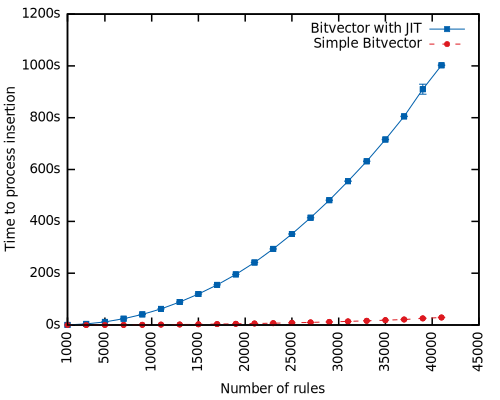
\includegraphics[height=0.9\textheight]{figures/eval_time}
\end{frame}

\begin{frame}
  Vergleich des Speicherverbrauchs:
  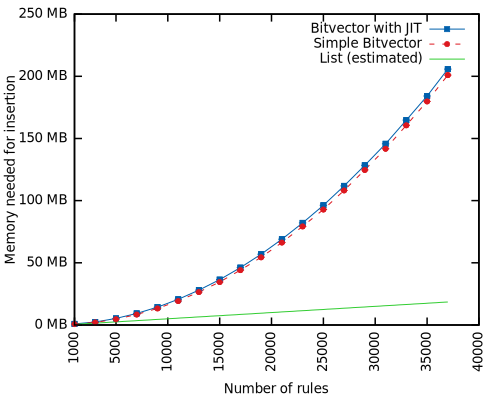
\includegraphics[height=0.9\textheight]{figures/eval_mem}
\end{frame}

\section{\scshape Fazit und Ausblick}
\begin{frame}
  \centering\Huge{\insertsection}
\end{frame}

\subsection{\scshape Allgemeine Ergebnisse}
\begin{frame}
  \begin{tcolorbox}[colback=teal!5!white,colframe=teal!75!black,title=Wichtigste Ergebnisse,drop fuzzy shadow]
    \begin{itemize}
      \item Verbesserung der Switch-Performance durch den Bitvector-Algorithmus.
      \item Implementierung eines Codegenerators für statische Regelsätze.
      \item Evaluation und Verifikation der neuen Komponenten.
    \end{itemize}
  \end{tcolorbox}
  \pause
  \begin{tcolorbox}[colback=blue!5!white,colframe=blue!75!black,title=Künftige Anknüpfungspunkte,drop fuzzy shadow]
    \begin{itemize}
      \item Inkrementelles Update der JIT-Funktion bei Regelsatzänderung.
      \item Optimierung der JIT-Funktion nach beobachteten Traffic-Mustern.
    \end{itemize}
  \end{tcolorbox}
\end{frame}

\section{}
\begin{frame}
  \frametitle{\scshape Fragen?}
  \centering\Huge{?}
\end{frame}

\appendix
\section{\scshape Weitere Ergebnisse}
\begin{frame}[noframenumbering]
  \frametitle{Aufteilung der Regelmenge}
  \centering\includegraphics[height=0.9\textheight]{figures/rule-thirds}
\end{frame}

\begin{frame}[noframenumbering]
  Ergebnisse für oberstes Drittel:
  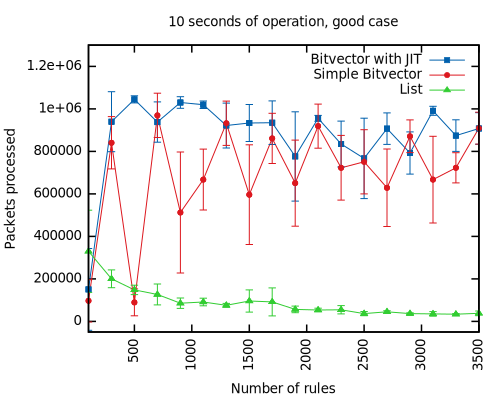
\includegraphics[height=0.9\textheight]{figures/eval_b}
\end{frame}

\begin{frame}[noframenumbering]
  Ergebnisse im mittleren Drittel:
  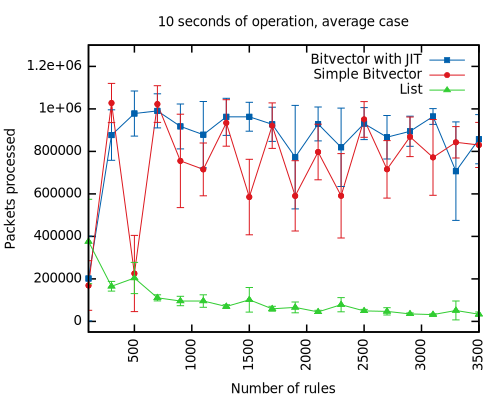
\includegraphics[height=0.9\textheight]{figures/eval_a}
\end{frame}

\begin{frame}[noframenumbering]
  Ergebnisse im letzten Drittel:
  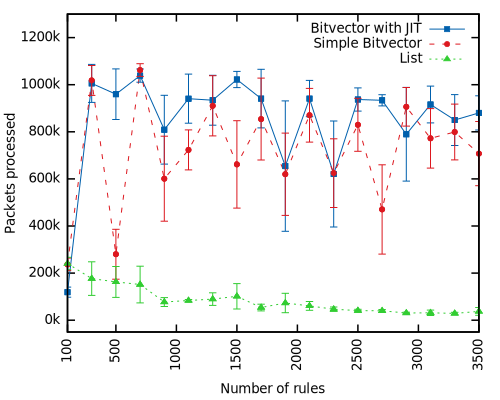
\includegraphics[height=0.9\textheight]{figures/eval_w}
\end{frame}

\begin{frame}[noframenumbering]
  Relative Verbesserung (oberstes Drittel):
  \includegraphics[height=0.9\textheight]{figures/eval_b_relative}
\end{frame}

\begin{frame}[noframenumbering]
  Relative Verbesserung (zweites Drittel):
  \includegraphics[height=0.9\textheight]{figures/eval_a_relative}
\end{frame}

\begin{frame}[noframenumbering]
  Relative Verbesserung (letztes Drittel):
  \includegraphics[height=0.9\textheight]{figures/eval_w_relative}
\end{frame}

\end{document}
